\chapter{Integration Tests}

\section{Test case scenarios}
\begin{table}[H]
    \begin{tabular}{|l|l|l|p{10cm}|}
    \hline
    Case & Control Unit & Unit under Test & Execution \\ \hline
    1 & CDU & Sensor & CDU sends a get data request to a sensor. \\ \hline
    2 & Sensor & CDU & Sensor sends data to the CDU \\ \hline
    3 & PC & CDU & PC sends a get data request to the CDU \\ \hline
    4 & CDU & Sensor & CDU requests data from a sensor that does not exists \\ \hline
    5 & PC & CDU & PC sends a message to the CDU that the CDU does not recognise. \\ \hline
    6 & Sensor & CDU & Sensor sends invalid data to the CDU \\ \hline
    7 & Sensor & CDU & CDU sends a get data request to a sensor but does not allow the sensor to respond. \\ \hline
    8 & Sensor & CDU & CDU sends a get data request to a sensor. The sensor responds but occupies the bus and never lets go. \\ \hline
    \end{tabular}
\end{table}

\section{Test case results}
\begin{table}[H]
    \begin{tabular}{|l|l|l|p{10cm}|}
    \hline
    Case & Expected result & Actual result & Done \\ \hline
    1 & ~ & ~ & ~\\ \hline
    2 & ~ & ~ & ~\\ \hline
    3 & ~ & ~ & ~\\ \hline
    4 & ~ & ~ & ~\\ \hline
    5 & ~ & ~ & ~\\ \hline
    6 & ~ & ~ & ~\\ \hline
    7 & ~ & ~ & ~\\ \hline
    8 & ~ & ~ & ~\\ \hline
    \end{tabular}
\end{table}

\chapter{Unit Tests}
%%%%%%%%%%%%%%%%%%%%%%%%%%%%%%%%%%%%%%%%%%%%%%%%%%%%%%%%%%%%%%%%%%%%%%%%%%%%%%%
%%%%%%%%%%%%%%%%%%%%%%%%%%%%%%% CDU %%%%%%%%%%%%%%%%%%%%%%%%%%%%%%%%%%%%%%%%%%%
%%%%%%%%%%%%%%%%%%%%%%%%%%%%%%%%%%%%%%%%%%%%%%%%%%%%%%%%%%%%%%%%%%%%%%%%%%%%%%%
\section{CDU}
%% The hardware tests of the CDU
This section contains the hardware and software unit tests of the CDU.
\subsection{Hardware}
In order to test the hardware of the CDU, a series of test points was put on the circuitry. External hardware will be needed for some tests. This will be stated clearly if needed.
\subsubsection{Test case 1: 3.3 volt power supply}
\textbf{Purpose:}\\
The purpose of this test is to test the 3.3 volt circuitry of the power supply block in the CDU.\\

\textbf{Test equipment:}
\begin{itemize}
\item Multimeter: Meterman 37XR
\item CDU (UUT)
\item Bus test stub
\end{itemize}

\textbf{Procedure:}\\
Apply 20 V on the P+ and P- pins. Measure voltage between 3v3TEST pin and GNDPIN with an oscilloscope.\\

\textbf{Expected Result:}\\
3.35$\pm$0.17 volts are measured.\\

\textbf{Actual Result:}\\
\begin{table}[H]
\centering
\begin{tabular}{|p{2cm}|p{2cm}|p{3cm}|p{2cm}|}\hline
\textbf{Test case:} & \textbf{Date:} & \textbf{Measurement:} & \textbf{Result:} \\ \hline
1 & 30-04-2014 & 3.36V & PASSED \\ \hline
\end{tabular}
\end{table}

\textbf{Comment and remarks:}\\
Well in range\\

\subsubsection{Test case 2: Communication to bus}
\textbf{Purpose:}\\
The purpose of this test is to test the communication to bus circuitry.\\

\textbf{Test equipment:}
\begin{itemize}
\item HAMEG HM203-6 Oscilloscope
\item HAMEG HM8030-3 Function generator
\item CDU (UUT)
\item Bus test stub
\end{itemize}

\textbf{Procedure:}\\
Apply 20 V on the P+ and P- pins. Between B+ and B- pins put a circuit of 4.7 volt Zener diode and a 5 ohm resistor. Apply 10 kHz signal to INPUTTEST pin. Observe AC coupled signal between SenseTEST pin and GNDPIN with an oscilloscope.\\

\textbf{Expected Result:}\\
10 kHz signal is observed.\\

\textbf{Actual Result:}\\
\begin{table}[H]
\centering
\begin{tabular}{|p{2cm}|p{2cm}|p{3cm}|p{2cm}|}\hline
\textbf{Test case:} & \textbf{Date:} & \textbf{Measurement:} & \textbf{Result:} \\ \hline
2 & 30-04-2014 & 10 kHz signal & PASSED \\ \hline
\end{tabular}
\end{table}

\textbf{Comment and remarks:}\\
-\\

\subsubsection{Test case 3: Voltage reference in receiver circuit}
\textbf{Purpose:}\\
The purpose of this test is to test the voltage reference in receiver circuitry.\\

\textbf{Test equipment:}
\begin{itemize}
\item Multimeter: Meterman 37XR
\item CDU (UUT)
\item Bus test stub
\end{itemize}

\textbf{Procedure:}\\
Apply 20 V on the P+ and P- pins. Between B+ and B- pins put a circuit of 4.7 volt Zener diode and a 5 ohm resistor. Measure voltage between REFTEST pin and GNDPIN with an oscilloscope.\\

\textbf{Expected Result:}\\
0.43$\pm$0.02 volts are measured.\\

\textbf{Actual Result:}\\
\begin{table}[H]
\centering
\begin{tabular}{|p{2cm}|p{2cm}|p{3cm}|p{2cm}|}\hline
\textbf{Test case:} & \textbf{Date:} & \textbf{Measurement:} & \textbf{Result:} \\ \hline
3 & 30-04-2014 & 0.44V & PASSED \\ \hline
\end{tabular}
\end{table}

\textbf{Comment and remarks:}\\
within range\\

\subsubsection{Test case 4: Communication from bus}
\textbf{Purpose:}\\
The purpose of this test is to test the communication from bus circuitry\\

\textbf{Test equipment:}
\begin{itemize}
\item HAMEG HM203-6 Oscilloscope
\item HAMEG HM8030-3 Function generator
\item CDU (UUT)
\item Bus test stub
\end{itemize}

\textbf{Procedure:}\\
Apply 20 V on the P+ and P- pins. Between B+ and B- pins put a circuit of 4.7 volt Zener diode, a 5 ohm resistor and a BAV21 diode and ZVN3306A. For clarification look at figure ~\ref{fig:busteststub}. Apply 10 kHz signal with the function generator to the ZVN3306A on the pins shown in the bus test stub figure. Observe AC signal between OUTPUTTEST pin and GNDPIN with the oscilloscope.\\
\begin{figure}[H]
\centering
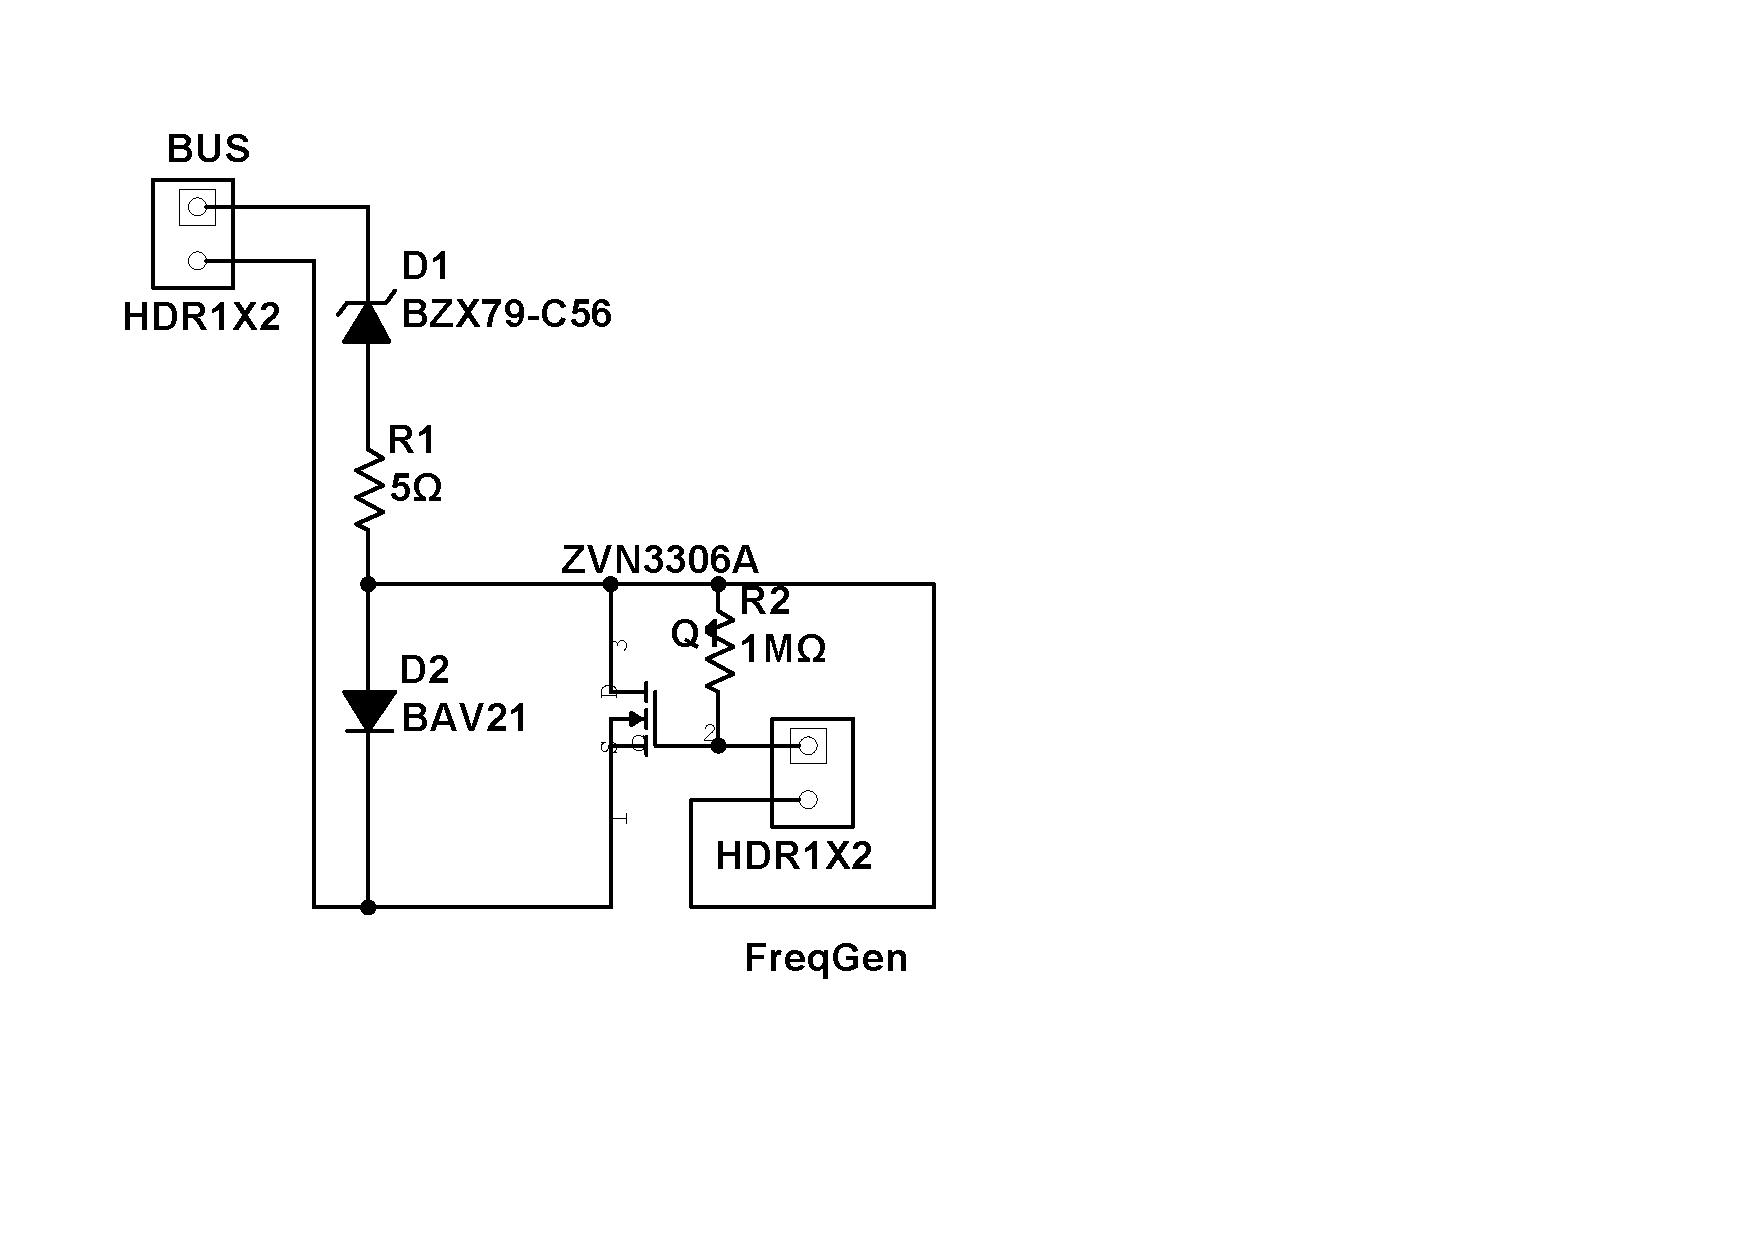
\includegraphics[width=0.8\textwidth]{billeder/BusTestStub}
\caption{Bus test stub}
\label{fig:busteststub}
\end{figure} 


\textbf{Expected Result:}\\
10 kHz signal is observed.\\

\textbf{Actual Result:}\\
\begin{table}[H]
\centering
\begin{tabular}{|p{2cm}|p{2cm}|p{3cm}|p{2cm}|}\hline
\textbf{Test case:} & \textbf{Date:} & \textbf{Measurement:} & \textbf{Result:} \\ \hline
4 & 30-04-2014 & 10 kHz signal & PASSED \\ \hline
\end{tabular}
\end{table}

\textbf{Comment and remarks:}\\
-\\

\subsection{Software}
The software tests of the CDU
\subsubsection{Test case 5: Test of function IntegerToBinary }
\textbf{Purpose:}\\
The purpose of this test is to test the function IntegerToBinary with the parameters: unsigned char input, unsigned char size, unsigned char* outputbuffer.\\

\textbf{Test equipment:}
\begin{itemize}
\item CDU (UUT)
\item MPLAB X IDE
\item Explorer 16 board
\item ICD 3 Debugger
\end{itemize}

\textbf{Procedure:}\\
Connect the Explorer 16 board to the ICD 3 Debugger. A test program inserts values into the function. The size of the outputbuffer and a pointer to the outputbuffer is inserted into the function as well. The outputbuffer must be large enough to contain the number! Standard size is 8 bit for unsigned char data type.\\
Verify the content of the outputbuffer with the the MPLAB X debugging feature. Values larger than zero and smaller than 255 will be converted to a bit string. 

\textbf{Expected Result:}\\
Values from 0 to 255  will be successfully converted to bit strings.\\

\textbf{Actual Result:}\\
\begin{table}[H]
\centering
\begin{tabular}{|p{2cm}|p{2cm}|p{3cm}|p{2cm}|}\hline
\textbf{Test case:} & \textbf{Date:} & \textbf{Measurement:} & \textbf{Result:} \\ \hline
5 & 01-05-2014 & See below & PASSED \\ \hline
\end{tabular}
\end{table}
Values from 0 to 255 was inserted into the outputbuffer. This was checked with the debugger.\\
\begin{figure}[H]
\centering
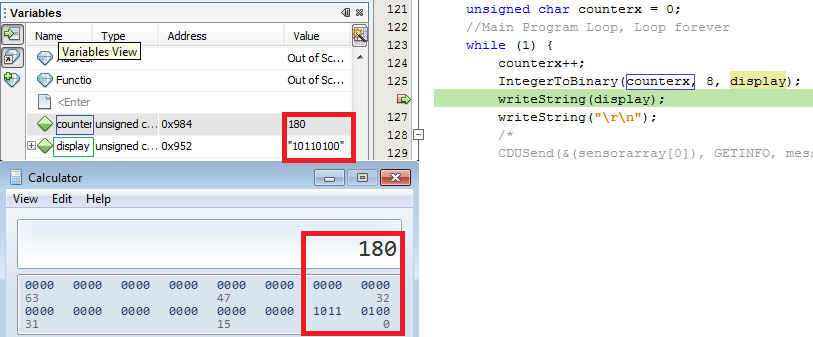
\includegraphics[width=0.8\textwidth]{billeder/CDUtestcase5}
\caption{Test Case 5 Result}
\label{fig:cdutestcase5}
\end{figure} 

\textbf{Comment and remarks:}\\
-\\

\subsubsection{Test case 6: Test of function PatMessage }
\textbf{Purpose:}\\
The purpose of this test is to test the function PatMessage with the parameters: unsigned char addr, unsigned char functioncode, unsigned char* outputbuffer.\\

\textbf{Test equipment:}
\begin{itemize}
\item CDU (UUT)
\item MPLAB X IDE
\item Explorer 16 board
\item ICD 3 Debugger
\end{itemize}

\textbf{Procedure:}\\
Connect the Explorer 16 board to the ICD 3 Debugger. A test program inserts addresses, function codes and a pointer to the outputbuffer is inserted into the function. The outputbuffer must be atleast 12 slots big.\\
Verify the content of the outputbuffer with the the MPLAB X debugging feature. The buffer must contain the start sequence, address and function code inserted into the function.\\

\textbf{Expected Result:}\\
The function should create the proper content as long as function code and address is within range. If address or function code is out of range the buffer will contain the start sequence and zeros.\\

\textbf{Actual Result:}\\
\begin{table}[H]
\centering
\begin{tabular}{|p{2cm}|p{2cm}|p{3cm}|p{2cm}|}\hline
\textbf{Test case:} & \textbf{Date:} & \textbf{Measurement:} & \textbf{Result:} \\ \hline
6 & 01-05-2014 & See below & PASSED \\ \hline
\end{tabular}
\end{table}
The correct address and function code was read from the outputbuffer. This is seen on figure ~\ref{fig:cdutestcase6}.\\
\begin{figure}[H]
\centering
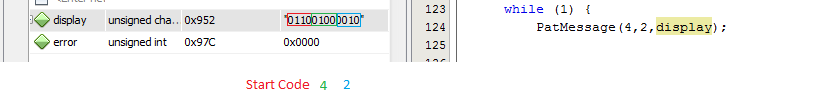
\includegraphics[width=1\textwidth]{billeder/CDUtestcase6}
\caption{Test Case 6 Result}
\label{fig:cdutestcase6}
\end{figure}

\textbf{Comment and remarks:}\\
-\\

\subsubsection{Test case 7: Test of function ToManchester }
\textbf{Purpose:}\\
The purpose of this test is to test the function ToManchester with the parameters: unsigned char* inputbuffer, unsigned char* outputbuffer, struct cduflags* CDUFlags.\\

\textbf{Test equipment:}
\begin{itemize}
\item CDU (UUT)
\item MPLAB X IDE
\item Explorer 16 board
\item ICD 3 Debugger
\end{itemize}

\textbf{Procedure:}\\
Connect the Explorer 16 board to the ICD 3 Debugger. A test message is loaded into an inputbuffer. The buffer is inserted into the function. An outputbuffer that has to be atleast twice the size of the inputbuffer is inserted as well. Lastly a cduflags struct is inserted. Verify that the outputbuffers content is a manchester coded equivalent to the input signal.\\

\textbf{Expected Result:}\\
The content of the outputbuffer is a manchester coded equivalent to the content of the inputbuffer loaded with the test message.\\

\textbf{Actual Result:}\\
\begin{table}[H]
\centering
\begin{tabular}{|p{2cm}|p{2cm}|p{3cm}|p{2cm}|}\hline
\textbf{Test case:} & \textbf{Date:} & \textbf{Measurement:} & \textbf{Result:} \\ \hline
7 & 01-05-2014 & See below & PASSED \\ \hline
\end{tabular}
\end{table}
The outputbuffer contains the the manchester coded equivalent to the content of the inputbuffer.\\

\begin{figure}[H]
\centering
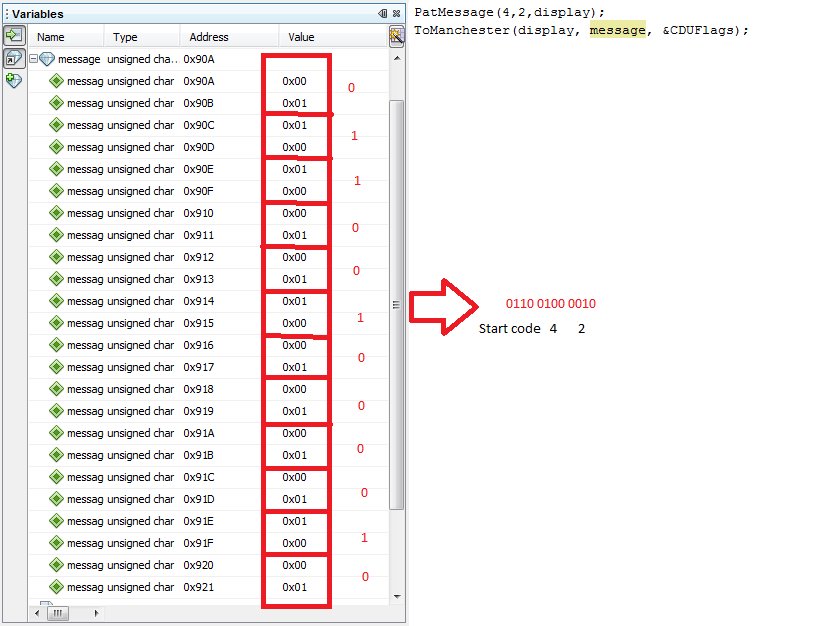
\includegraphics[width=1\textwidth]{billeder/CDUtestcase7}
\caption{Test Case 7 Result}
\label{fig:cdutestcase7}
\end{figure}

\textbf{Comment and remarks:}\\
-\\

\subsubsection{Test case 8: Test of function InitSensorArray }
\textbf{Purpose:}\\
The purpose of this test is to test the function InitSensorArray with the parameter: Sensor* sensorarray.\\

\textbf{Test equipment:}
\begin{itemize}
\item CDU (UUT)
\item MPLAB X IDE
\item Explorer 16 board
\item ICD 3 Debugger
\end{itemize}

\textbf{Procedure:}\\
Connect the Explorer 16 board to the ICD 3 Debugger. A sensorarray with defined slots is inserted into the function. After the function has been run, check the address of every sensor in the array. Addresses from 1 to 15 should be observed. Sensors after 15 in the array will not be initiated.\\

\textbf{Expected Result:}\\
The sensors in the array have been initiated with addresses from 1 to 15.\\

\textbf{Actual Result:}\\
\begin{table}[H]
\centering
\begin{tabular}{|p{2cm}|p{2cm}|p{3cm}|p{2cm}|}\hline
\textbf{Test case:} & \textbf{Date:} & \textbf{Measurement:} & \textbf{Result:} \\ \hline
8 & 01-05-2015 & See below & PASSED \\ \hline
\end{tabular}
\end{table}
The sensors in the array have been initiated properly.\\
\begin{figure}[H]
\centering
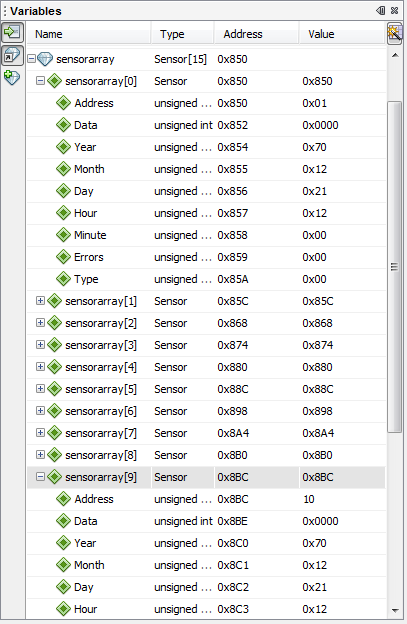
\includegraphics[width=0.5\textwidth]{billeder/CDUtestcase8}
\caption{Test Case 8 Result}
\label{fig:cdutestcase8}
\end{figure}

\textbf{Comment and remarks:}\\
-\\

\subsubsection{Test case 9: Test of function CDUSend }
\textbf{Purpose:}\\
The purpose of this test is to test the function CDUSend with the parameters: Sensor* Sens, unsigned char functioncode, unsigned char* Messagebuffer, struct cduflags* CDUFlags.\\

\textbf{Test equipment:}
\begin{itemize}
\item CDU (UUT)
\item MPLAB X IDE
\item Explorer 16 board
\item ICD 3 Debugger
\item HAMEG HM203-6 Oscilloscope
\end{itemize}

\textbf{Procedure:}\\
Connect the Explorer 16 board to the ICD 3 Debugger. Insert a sensor, a functioncode, a messagebuffer and a cduflags struct point into the function. Verify on an oscilloscope that a message was sent by observing on PORTA5 and GND.\\

\textbf{Expected Result:}\\
A message was observed on PORTA5. Message corresponds to inserted sensor and functioncode.\\

\textbf{Actual Result:}\\
\begin{table}[H]
\centering
\begin{tabular}{|p{2cm}|p{2cm}|p{3cm}|p{2cm}|}\hline
\textbf{Test case:} & \textbf{Date:} & \textbf{Measurement:} & \textbf{Result:} \\ \hline
9 & - & - & - \\ \hline
\end{tabular}
\end{table}

\textbf{Comment and remarks:}\\
-\\

\subsubsection{Test case 10: Test of function CDUReceive }
\textbf{Purpose:}\\
The purpose of this test is to test the function CDUReceive with the parameters: Sensor* Sens, unsigned char functioncode, unsigned char* receivebuffer, struct cduflags* CDUFlags and the return type unsigned char.\\

\textbf{Test equipment:}
\begin{itemize}
\item CDU (UUT)
\item MPLAB X IDE
\item Explorer 16 board
\item ICD 3 Debugger
\end{itemize}

\textbf{Procedure:}\\
Connect the Explorer 16 board to the ICD 3 Debugger. Create 2 testbuffers. One with a correct message and wrong with a message containing errors. Insert a sensor, a function code, one of the testbuffers and a cduflags struct pointer. Set the recvflag to 1. Observe the returned unsigned char and sensor struct. Switch the testbuffer and observe the returned unsigned char and sensor struct.\\

\textbf{Expected Result:}\\
When inserting a buffer containing a correct message, the returned unsigned char will be 1. The sensor struct is updated containing the data from the message.\\
When inserting a buffer containing a message with errors, the returned unsigned char will be 0. The sensor struct is not updated.\\

\textbf{Actual Result:}\\
\begin{table}[H]
\centering
\begin{tabular}{|p{2cm}|p{2cm}|p{3cm}|p{2cm}|}\hline
\textbf{Test case:} & \textbf{Date:} & \textbf{Measurement:} & \textbf{Result:} \\ \hline
9 & - & - & - \\ \hline
\end{tabular}
\end{table}

\textbf{Comment and remarks:}\\
-\\

%%%%%%%%%%%%%%%%%%%%%%%%%%%%%%%%%%%%%%%%%%%%%%%%%%%%%%%%%%%%%%%%%%%%%%%%%%%%%%%
%%%%%%%%%%%%%%%%%%%%%%%%%%%%%%% SN %%%%%%%%%%%%%%%%%%%%%%%%%%%%%%%%%%%%%%%%%%%%
%%%%%%%%%%%%%%%%%%%%%%%%%%%%%%%%%%%%%%%%%%%%%%%%%%%%%%%%%%%%%%%%%%%%%%%%%%%%%%%
\section{Sensor Node}
\subsection{Hardware}
The hardware tests of the Sensor node
\subsubsection{Test case 1: 3.3 volt power supply}
\textbf{Purpose:}\\
The purpose of this test is to test the 3.3 volt circuitry of the power supply block in the sensor node.\\

\textbf{Test equipment:}
\begin{itemize}
\item Multimeter: Meterman 37XR
\item Sensor node (UUT)
\item Sensor node supply test stub
\end{itemize}
\ \\
\textbf{Procedure:}\\
Connect B+ from the sensor node supply test stub (see figure \ref{fig:sensor_node_supply_test_Stub}) to the S+ on the UUT. Connect B- from the sensor node supply test stub to the S- on the UUT.\\
Measure the voltage from the GND testpin to the 3V3 testpin.

\begin{figure}[H]
	\centering
	\subbottom[Sensor node supply test stub]{%
		\includegraphics[width=.48\linewidth]{billeder/sensor_node_supply_test_stub}}
	\subbottom[Picture of the sensor node]{%
		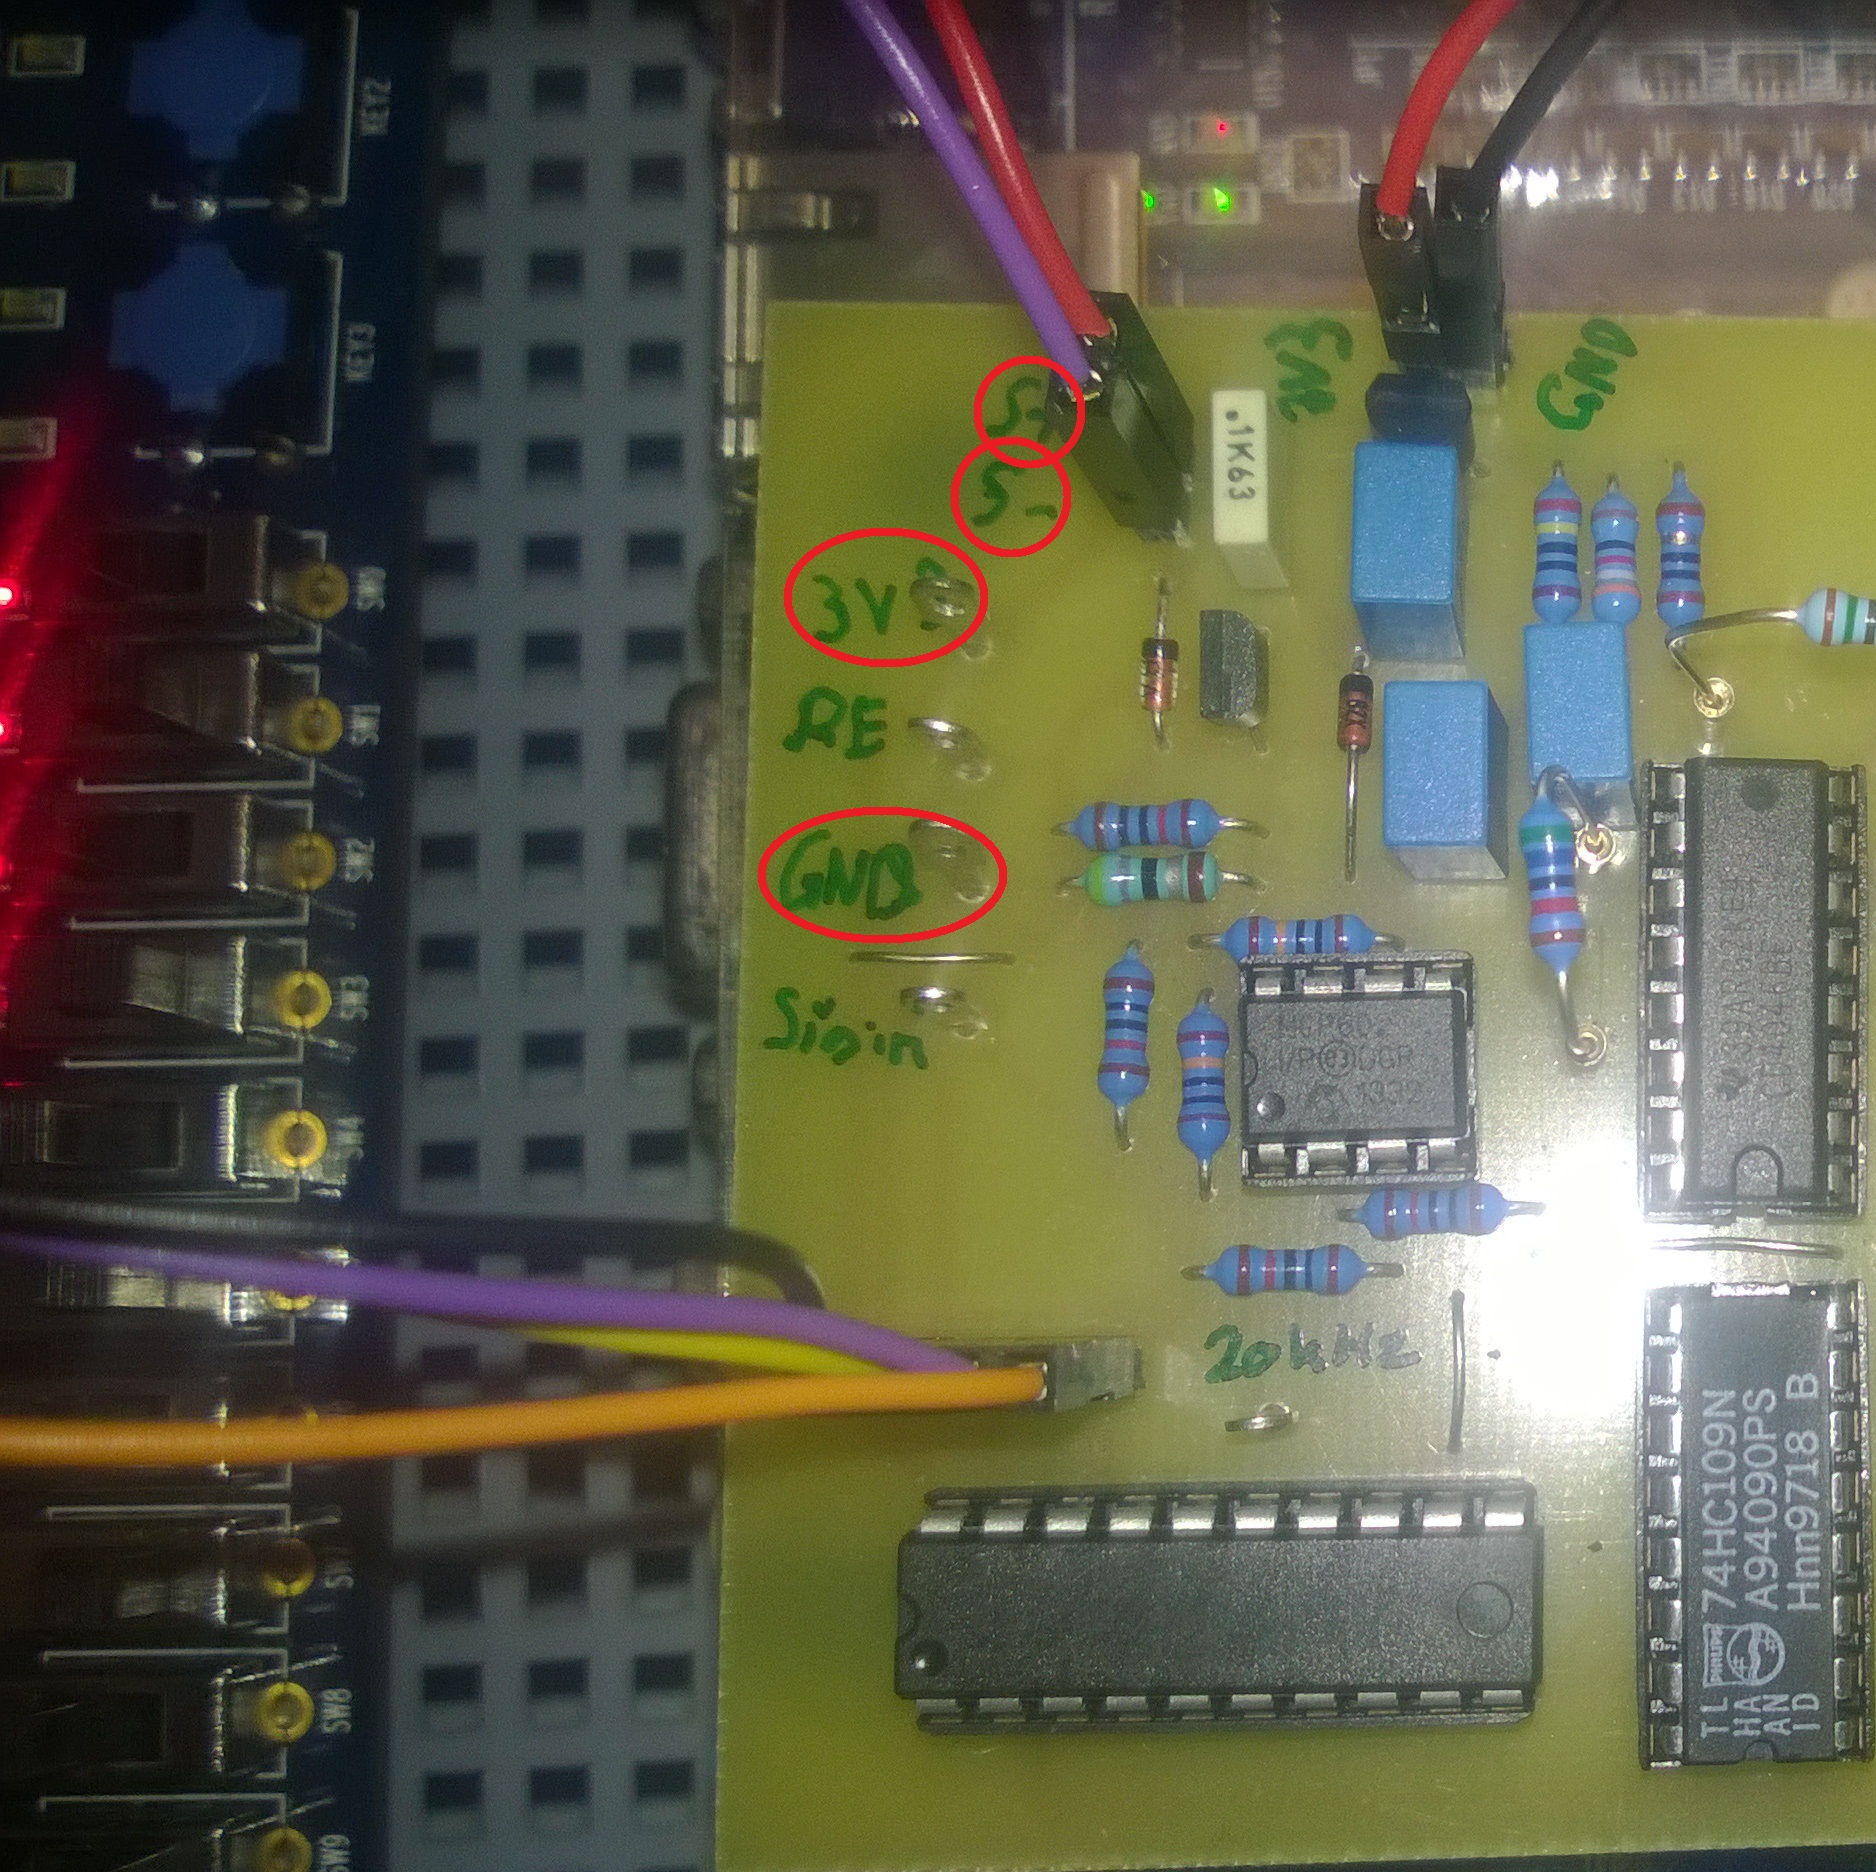
\includegraphics[width=.48\linewidth]{billeder/case5_picture}}

%\label{fig:sensor_node_supply_test_Stub}
%\end{subfigure}
\end{figure}

\textbf{Expected Result:}\\
3.35V$\pm$0.17V are measured.\\

\textbf{Result:}
\begin{table}[H]
\centering
\begin{tabular}{|p{2cm}|p{3cm}|p{2cm}|}\hline
\textbf{Date:} & \textbf{Measurement:} & \textbf{Result:} \\ \hline
30-04-2014 & 3.30V & PASSED \\ \hline
\end{tabular}
\end{table}

\textbf{Comment and remarks:}\\
-\\

\subsubsection{Test case 2: Data recovery circuit}
\textbf{Purpose:}\\
The purpose of this test is to test the data recovery circuit located on the sensor node.  The levels and frequency must not vary more then specified in the implementation documentation.\\

\textbf{Test equipment:}
\begin{itemize}
\item Analog Discovery USB oscilloscope
\item HAMEG HM8030-3 Function generator
\item Sensor node (UUT)
\item Sensor node communication stub
\end{itemize}
\ \\
\textbf{Procedure:}\\
Connect B+ from the sensor node communication test stub to the S+ on the UUT. Connect B- from the sensor node communication test stub to the S- on the UUT.
Connect FG+ from the sensor node communication test stub to the positive connector on the Function generator. Connect FG- from the sensor node communication test stub to the negative connector on the Function generator.\\ Set the Function generator to:
\begin{itemize}
\item pk-pk: 3.3V
\item DC offset: 1.65V
\item frequency: 10kHz
\item Waveform: Square
\end{itemize}
Connect the oscilloscope ground to the GND test point on the UUT.
Connect the oscilloscope probe to the DIN point on the UUT.\\
Set the Oscilloscope to:
\begin{itemize}
\item Volts/div: 1V
\item Time/div: 50$\mu$s
\item Probe: AC coupled
\end{itemize}
\begin{figure}[H]
	\centering
	\subbottom[Sensor node supply test stub]{%
		\includegraphics[width=.48\linewidth]{billeder/sensor_node_communication_test_stub}}
	\subbottom[Picture of the sensor node]{%
		\includegraphics[width=.48\linewidth]{billeder/case6_picture}}
\end{figure}

\textbf{Expected Result:}\\
Frequency: 10kHz\\
Amplitude: 3.3V$\pm$0.17V\\
Store a picture of the oscilloscope as reference.


\textbf{Result:}
\begin{table}[H]
\centering
\begin{tabular}{|p{2cm}|p{3cm}|p{2cm}|}\hline
\textbf{Date:} & \textbf{Measurement:} & \textbf{Result:} \\ \hline
--- & --- & --- \\ \hline
\end{tabular}
\end{table}
\textbf{Picture:}
\textbf{Comment and remarks:}\\
-\\

\subsubsection{Test case 3: Phase lock circuit}
\textbf{Purpose:}\\
The purpose of this test is to test the clock recovery circuit located on the sensor node. The levels and frequency must not vary more then specified in the implementation documentation.\\

\textbf{Test equipment:}
\begin{itemize}
	\item Analog Discovery USB oscilloscope
	\item HAMEG HM8030-3 Function generator
	\item Sensor node (UUT)
	\item Sensor node communication stub
\end{itemize}
\ \\
\textbf{Procedure:}\\
Connect B+ from the sensor node communication test stub to the S+ on the UUT. Connect B- from the sensor node communication test stub to the S- on the UUT.
Connect FG+ from the sensor node communication test stub to the positive connector on the Function generator. Connect FG- from the sensor node communication test stub to the negative connector on the Function generator.\\ Set the Function generator to:
\begin{itemize}
	\item pk-pk: 3.3V
	\item DC offset: 1.65V
	\item frequency: 10kHz
	\item Waveform: Square
\end{itemize}

Connect the oscilloscope ground to the GND test point on the UUT.
Connect the oscilloscope probe 1 to the DIN point on the UUT.
Connect the oscilloscope probe 2 to the 10kHz test point on the UUT.\\
Set the Oscilloscope to:
\begin{itemize}
	\item Volts/div: 1V
	\item Time/div: 50$\mu$s
	\item Probe: AC coupled
\end{itemize}

\begin{figure}[H]
	\centering
	\subbottom[Sensor node supply test stub]{%
		\includegraphics[width=.48\linewidth]{billeder/sensor_node_communication_test_stub}}
	\subbottom[Picture of the sensor node]{%
		\includegraphics[width=.48\linewidth]{billeder/case6_picture}}
\end{figure}

\textbf{Expected Result:}\\
Frequency: 10 kHz locked in 90$^\circ$ phase with the input signal.\\
Store a picture of the oscilloscope as reference.


\textbf{Result:}
\begin{table}[H]
	\centering
	\begin{tabular}{|p{2cm}|p{3cm}|p{2cm}|}\hline
		\textbf{Date:} & \textbf{Measurement:} & \textbf{Result:} \\ \hline
	 	01-05-2014 & See scope picture & PASSED \\ \hline
	\end{tabular}
\end{table}
\textbf{Picture:}
\begin{figure}[H]
\centering
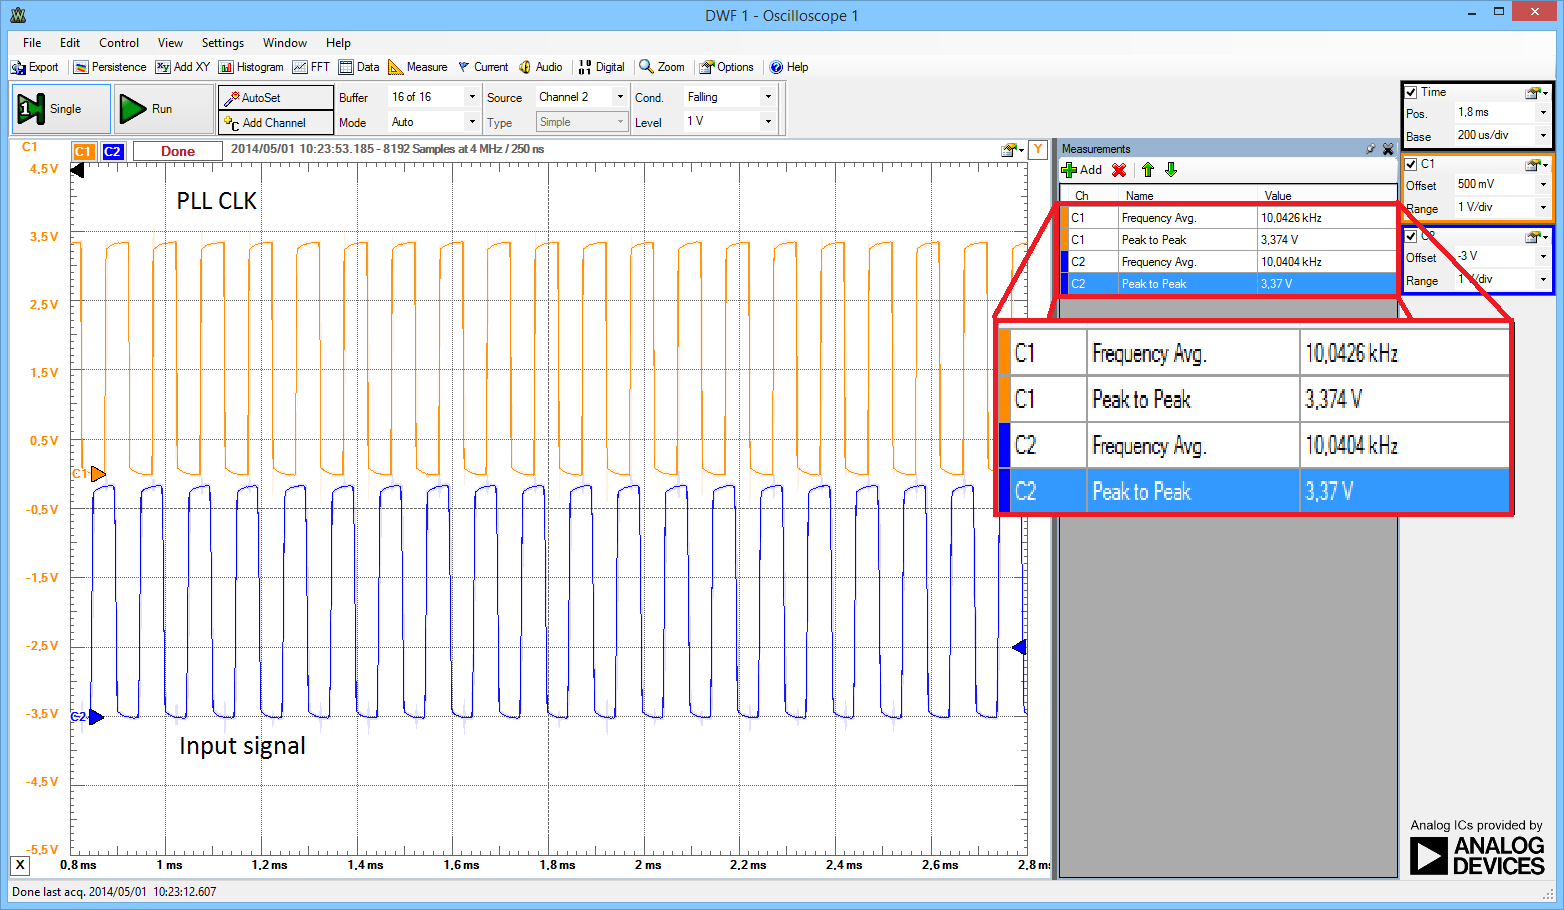
\includegraphics[width=.9\textwidth]{billeder/SN_Case_2_osc_picture}
\end{figure}
\textbf{Comment and remarks:}\\
-\\

\subsection{Software}
The software tests of the Sensor node